\subsection{Continuous liftings of étale maps}

Let \(p \colon \mathrm{E} \to \mathrm{B}\) and \(f \colon \mathrm{Z} \to \mathrm{B}\) be continuous maps. A continuous lifting of \(f\) to \(\mathrm{E}\) is called a continuous map \(g \colon \mathrm{Z} \to \mathrm{E}\) such that \(p \circ g = f\). The set of continuous liftings of \(f\) to \(\mathrm{E}\) is none other than \(\mathcal{C}_{\mathrm{B}}(\mathrm{Z};\mathrm{E})\). It is also identified with the set \(\mathcal{S}(\mathrm{Z};\mathrm{Z} \times_{\mathrm{B}}\mathrm{E})\) of continuous sections of the projection of the Z-space \((\mathrm{Z} \times_{\mathrm{B}}\mathrm{E},\mathrm{pr}_{1})\).

If T is a subset of Z, a continuous lifting of f to E defined on T is called a continuous lifting of f \textbar{} T to E:

\pandocbounded{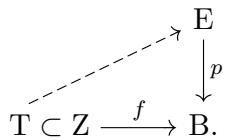
\includegraphics[keepaspectratio]{images/part001_46887bc2.jpg}}

PROPOSITION 10. --- Let E, B and Z be topological spaces, \(p\colon E \to B\) an étale map and \(f\colon Z \to B\) a continuous map.

Let \(z \in \mathbf{Z}\) and \(x \in \mathrm{E}\) be points such that \(f(z) = p(x)\). There exists a neighborhood \(\mathrm{W}\) of \(z\) on \(\mathbf{Z}\) and a continuous lifting \(g\) of \(f\) to \(\mathrm{E}\), defined on \(\mathrm{W}\), such that \(g(z) = x\).

There exists an open neighborhood V of \(p(x)\) in B and a continuous section s of p over V such that \(s(p(x)) = x\) (Proposition 9). The set \(W = f^{-1}(V)\) is an open neighborhood of z and the map \(g = s \circ (f|W)\) is a continuous lifting of f to E, defined on W and such that \(g(z) = x\).

PROPOSITION 11. --- Let E, B, and Z be topological spaces, let \(p\colon E \to B\) and \(f\colon Z \to B\) be continuous maps. Let \(g\) and \(g'\) be continuous liftings of \(f\) to E. Let W be the set of points of Z where \(g\) and \(g'\) coincide.

\begin{enumerate}
\def\labelenumi{\alph{enumi})}
\item
  If the map p is separated, W is closed.
\item
  If the map p is étale, W is open.
\end{enumerate}

Denote by \(h\) the continuous map \((g, g')\colon Z \to E \times E\). The image of \(h\) is contained in \(E \times_{B} E\) since \(p \circ g = f = p \circ g'\), and the set W of points of Z where g and g' coincide is the inverse image under \(h\) of the diagonal \(\Delta_{E}\).

If the map p is étale, the diagonal \(\Delta_{E}\) is open in \(E \times_{B} E\) (I, p. 31, prop. 7), hence the set W is open in Z.

If the map p is separated, the diagonal \(\Delta_{E}\) is closed in \(E \times_{B} E\) (I, p. 25, def. 1) and the set W is closed in Z.

COROLLARY 1. --- If the space Z is connected and if the map p is étale and separated, then continuous liftings of f to E that coincide at one point are equal.

COROLLARY 2. --- Let \(p\colon E \to B\) be a separated étale map. If the space E is connected, the group \(\mathrm{Aut}_{\mathrm{B}}(\mathrm{E})\) acts freely on E.

Indeed, if \(f: \mathrm{E} \to \mathrm{E}\) is a B-morphism, the set of points where f and \(\mathrm{Id}_{\mathrm{E}}\) coincide is E or the empty set by Cor. 1.

COROLLARY 3. --- Let E, B, and Z be topological spaces, let \(p\colon E \to B\) be a separated étale morphism, and let \(f\colon Z \to B\) be a continuous map. For \(i = 1,2\), let \(U_i\) be an open (resp. closed) subset of Z and \(g_i\colon U_i \to E\) be a continuous lifting of f defined on \(U_i\). Assume that the intersection \(U_1 \cap U_2\) is connected and that there exists a point z of \(U_1 \cap U_2\) such that \(g_1(z) = g_2(z)\). Then there exists a continuous lifting of f defined on \(U_1 \cup U_2\) which extends \(g_1\) and \(g_2\).

By corollary 1, the restrictions to \(U_{1} \cap U_{2}\) of \(g_{1}\) and \(g_{2}\) are equal. The map \(g: U_{1} \cup U_{2} \to E\) defined by \(g(z) = g_{i}(z)\) for \(z \in U_{i}\) (i = 1, 2) is a continuous lifting of f defined on \(U_{1} \cup U_{2}\) (TG, I, p. 19, prop. 4).

In the preceding results, the special case where Z = B and \(f = Id_{B}\) is important: the continuous liftings of f are then the continuous sections of p.

PROPOSITION 12. --- Let \(p \colon E \to B\) be an étale map. For the map \(p\) to be separated, it is necessary and sufficient that for every open subset \(V\) of \(B\) and every pair \((s, s')\) of continuous sections of \(p\) over \(V\), the set of points where \(s\) and \(s'\) coincide be closed in \(V\).

The condition is necessary (Proposition 11, I, p. 34). Let us prove that it is sufficient. Let \(b\) be a point of B, and let \(x\) and \(x'\) be two distinct points of E such that \(p(x) = p(x') = b\). Let V be an open neighborhood of b and s, s' continuous sections of p over V such that \(s(\mathrm{V})\) and \(s'(\mathrm{V})\) are open neighborhoods of x and x', respectively (Proposition 9). By hypothesis, the set W of points \(x \in \mathrm{V}\) such that \(s(x) \ne s'(x)\) is open in V, hence in B. The sets \(s(\mathrm{W})\) and \(s'(\mathrm{W})\) are open neighborhoods of x and x', respectively; they are disjoint by construction. This proves that the map p is separated (I, p. 25, Definition 1).
% semantic-fragments: legacy-input-seam
\relax{}
